\section{Testing and Experimentation}\label{sec:testing-and-experimentation}

\subsection{Testing and Experiment Scope}\label{subsec:testing-and-experiment-scope}

With respect to the hardware, there were different approaches
to testing and experimentation
at different stages of development.
The following provides an overview of the different objectives that were present during each stage of development:

\begin{table}[htbp]
      \begin{center}
            \begin{tabular}{|p{0.2\linewidth}|p{0.6\linewidth}|}
                  \hline
                  \tablex{Ideation}{
                        -- Maximize performance to power ratio.\newline
                        -- Create a short list of configurations to further test during the assembly process.
                  }
                  \tablex{Assembly}{
                        -- Make use of the breadboard to physically explore configurations.\newline
                        -- Settle on one configuration after testing has been accomplished for the shortlisted configurations.
                  }
                  \tablex{Prototyping}{
                        -- Solder parts and check continuity after soldering.\newline
                        -- Explore soldering parts together to make servicing easier by reducing the number of connections between components.\newline
                        -- Make light considerations of accessibility/repairability when soldering parts together.
                  }                                                                                                                
                  \tablex{Finalizing}{
                        -- Solder parts in a manner that conserves space for the hardware enclosure.\newline
                        -- Make compromise between spatial compression and ease of repair.
                  }                                                                                                             
            \end{tabular}
      \end{center}
      \caption{Hardware Development Stages}
  \end{table}

As far as the software, a systematic approach was taken to ensure the
robustness and efficiency of the application.
The following objectives guided the testing and experimentation at various stages of development:

\begin{table}[htbp]
      \begin{center}
            \begin{tabular}{|p{0.2\linewidth}|p{0.7\linewidth}|}
                  \hline
                  \tablex{Research}{
                        -- Conduct Market Research.\newline
                        -- Identify key challenges to state-of-the-art.\newline
                        -- Conduct contemporary literature review.
                  }
                  \tablex{Ideation}{
                        -- Brainstorm a variety of potential solutions.\newline
                        -- Shortlist a few of the aforementioned solutions.\newline
                        -- Create possible architectures for front and back ends of application.\newline
                        -- Create low-fidelity proof-of-concept.
                  }
                  \tablex{Implementation}{
                        -- Choose one configuration of tools and technologies\newline
                        -- Create high-fidelity prototype by implementing certain features in an agile fashion\newline
                        -- Leverage developers to test for function first, then optimization second
                  }         
                  \tablex{Benchmarking}{
                        -- Emphasize optimization of the code and robustness\newline
                        -- Achieve a code coverage of at least 80 percent\newline
                        -- Reduce test case excapes to zero
                  }                                                                                                       
                  \tablex{Finalizing}{
                        -- Make cosmetic changes to the application\newline
                        -- Create script for live demonstration rehearsal\newline
                        -- Repeatedly test the system to ensure stability and consistency over time.
                  }                                                                                                             
            \end{tabular}
      \end{center}
      \caption{Software Development Stages}
  \end{table}

\subsection{Testing and Experiment Approach}\label{subsec:testing-and-experiment-approach}

% Hardware

Testing the hardware was an iterative process that entailed using simulations, continuity
checks, and constant soldering of different parts in different ways to conserve space to
make the hardware as physically unobtrusive as possible while keeping it easy to repair.
During the ideation phase, simulations were used with the Fritzing software where
different power deliveries and wiring configurations were tested via virtual
simulations.
This led to some of the compromises made as described in \textbf{Design Constraints, Problems, Trade-offs, and Solutions.}

During the assembly phase, a breadboard was used to test without spending time and
effort soldering and desoldering the configuration.
Once the hardware configuration reached a satisfactory level of performance, only then were the parts soldered
together.
During the prototyping phase, different wires and connectors were used to determine the best manner of mounting different components to one continuous
connection.
A proof of concept was made that had no consideration for conservation of space, and continuity checks were done with a multimeter to ensure that each
solder connection was made properly.

In finalizing the hardware configuration, several spare parts were soldered together
and connected onto the board that used different techniques to conserve space.
Again, the solder joints were tested for continuity with a multimeter.
In addition to conserving space, an additional consideration was made to avoid short-circuits
by exploring both electrical tape and heatshrink.
From there, ease of repair was taken into account by documenting the nature of the solder joints so end users
could easily replicate the consolidation done by the hardware system integrators.

% Software

In testing the software implementation, the primary goal was to validate the functionality,
reliability, and performance of the system across various components and integrations. %
The testing process was comprehensive, covering both unit and integration levels to
ensure the smooth functioning of individual elements as well as their
seamless integration into the whole system. %

The unit testing phase involved meticulously testing each system component in isolation,
scrutinizing the functions and methods within the Python and Flask backend, along
with the ReactJS frontend. %
The developers conducted a thorough examination of the functionality of MySQL database interactions and confirmed the dependable data
transmission between the microcontroller and the backend server using MicroPython. %

Integration testing was then conducted to secure a seamless connection between
the frontend, backend, and database, which guaranteed a consistent and accurate
flow of data. %
Validation was done by examining the communication efficiency between the microcontroller, sensors, and backend server, ensuring that the entire system
operated seamlessly when all components were brought together. %

\subsection{Testing and Experiment Results and Analysis}\label{subsec:testing-and-experiment-results-and-analysis}

While the majority of test cases passed successfully, demonstrating the system’s
robustness and reliability, any failed tests were promptly addressed,
with bugs fixed and tests rerun until success was achieved. %

\begin{itemize}
    \item \textbf{Performance Test Result Analysis}: The system performed well
          under normal conditions and was able to handle load up to performance benchmarks. %
    \item \textbf{Test Coverage}: To ensure confidence in the system’s reliability,
          tests achieved high coverage across the codebase. %
    \item \textbf{Bug Distribution Report}: Bugs were categorized based on their
          severity, with critical and major bugs given priority in fixing.  %
          GitHub Issues detailing of bugs, their severity, and the components
          they affected was created. %
\end{itemize}

\begin{figure}[htbp]
    \centering
    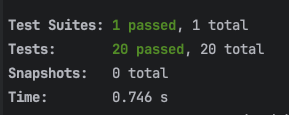
\includegraphics[width=1\linewidth]{datasets/images/Jest-Test-Suite.png}
    \caption{Using Jest Test Suite}
    \label{fig:figure2}

\end{figure}

\begin{figure}[htbp]
    \centering
    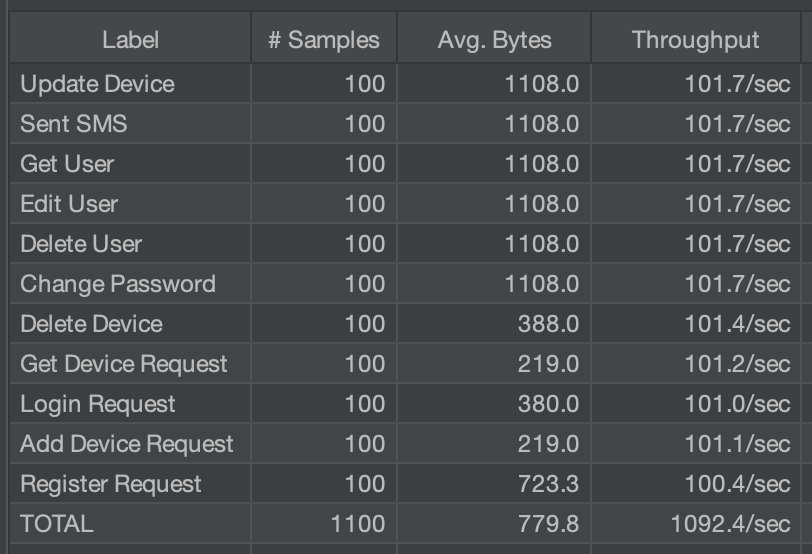
\includegraphics[width=1\linewidth]{datasets/images/JMeter_100reqBenchmark.png}
    \caption{JMeter 100 Request Benchmark Metrics}
    \label{fig:figure3}
\end{figure}

\begin{figure}[htbp]
    \centering
    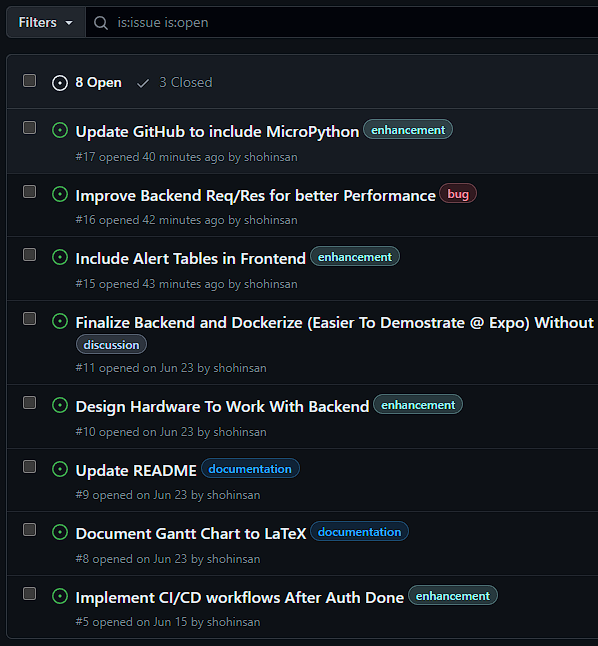
\includegraphics[width=1\linewidth]{datasets/images/GitHubIssues.png}
    \caption{Issue Tracking System}
    \label{fig:gitIssues}
\end{figure}

By rigorously following this comprehensive testing and experiment
approach, the developers ensured that the system was reliable,
performed well, and met all the defined requirements and benchmarks. %